% =====================================================================
%  Rapport de synthèse (6 à 10 pages) — « Prédiction de la qualité des soudures »
%  Compilation : tectonic rapport_final.tex
%  (ou pdflatex rapport_final → bibtex rapport_final → pdflatex ×2)
%  Réutilise le préambule, les figures et la bibliographie du rapport complet.
% =====================================================================
\documentclass[11pt,a4paper]{article}

% =====================================================================
%  Informations de la page de garde — à vérifier / compléter par l'équipe
%  Les éléments non connus sont affichés en rouge via \acompleter{...}.
% =====================================================================

\newcommand{\TitreRapport}{Prédiction de la qualité des soudures d'acier à partir de la Cambridge Weld Database}
\newcommand{\SousTitreRapport}{Rapport complet : de l'analyse exploratoire à l'analyse des résultats d'entraînement}
\newcommand{\TitreCourt}{Prédiction de la qualité des soudures --- rapport complet}

\newcommand{\Etablissement}{CentraleSupélec}
\newcommand{\Cours}{Projet de Machine Learning}
\newcommand{\NumeroEquipe}{\acompleter{numéro d'équipe}}
\newcommand{\DateRapport}{\today}

% Auteurs et adresses (reprises du rapport v1 du dépôt ; à vérifier).
\newcommand{\AuteurUn}{Mohamed SALH}
\newcommand{\MailUn}{mohamed.salh@student-cs.fr}
\newcommand{\AuteurDeux}{Mohamed CHEBLI}
\newcommand{\MailDeux}{mohamed.chebli@student-cs.fr}
\newcommand{\AuteurTrois}{Idriss BEN LETAIFA}
\newcommand{\MailTrois}{idriss.benletaifa@student-cs.fr}
\newcommand{\AuteursPDF}{Mohamed SALH, Mohamed CHEBLI, Idriss BEN LETAIFA}

\renewcommand{\SousTitreRapport}{Rapport de synthèse}
\renewcommand{\TitreCourt}{Prédiction de la qualité des soudures --- rapport de synthèse}
% =====================================================================
%  Préambule du rapport — compatible pdfLaTeX (Overleaf) et XeLaTeX
% =====================================================================

% ---------- Encodage et polices -------------------------------------
\usepackage{iftex}
\ifPDFTeX
  \usepackage[utf8]{inputenc}
  \usepackage[T1]{fontenc}
  \usepackage{lmodern}
  \usepackage{textcomp}
\else
  \usepackage{fontspec}
\fi
\usepackage[french]{babel}
% Légendes « Figure »/« Tableau » sans petites capitales (absentes en gras).
\ifdefined\frenchsetup\frenchsetup{SmallCapsFigTabCaptions=false}\fi
\AtBeginDocument{\renewcommand{\figurename}{Figure}\renewcommand{\tablename}{Tableau}%
  \renewcommand{\listtablename}{Liste des tableaux}}
\usepackage{microtype}

% ---------- Mise en page --------------------------------------------
\usepackage[a4paper,margin=2.3cm,headheight=28pt,includehead,includefoot]{geometry}
\usepackage{setspace}
\setstretch{1.08}
\usepackage{parskip}
\setlength{\emergencystretch}{2.5em} % évite les débordements de lignes
\setlength{\parskip}{0.55em}
\usepackage{enumitem}
\setlist{itemsep=0.15em,topsep=0.3em}

% ---------- Couleurs (charte CentraleSupélec, d'après le logo) ------
\usepackage[table]{xcolor}
\definecolor{csbordeaux}{HTML}{7C2E40}
\definecolor{csgris}{HTML}{6F6A7E}
\definecolor{csgrisclair}{HTML}{F2F1F4}
\definecolor{bleuviz}{HTML}{2A78D6}
\definecolor{orangeviz}{HTML}{EB6834}
\definecolor{vertviz}{HTML}{1BAF7A}
\definecolor{encre}{HTML}{0B0B0B}
\definecolor{encre2}{HTML}{52514E}
\definecolor{alerte}{HTML}{C0392B}

% ---------- Titres de sections --------------------------------------
\usepackage{titlesec}
\titleformat{\section}{\Large\bfseries\color{csbordeaux}}{\thesection}{0.8em}{}
\titleformat{\subsection}{\large\bfseries\color{csbordeaux!85!black}}{\thesubsection}{0.8em}{}
\titleformat{\subsubsection}{\normalsize\bfseries\color{csgris!80!black}}{\thesubsubsection}{0.8em}{}
\titlespacing*{\section}{0pt}{1.4em}{0.7em}
\titlespacing*{\subsection}{0pt}{1.1em}{0.4em}
\titlespacing*{\subsubsection}{0pt}{0.9em}{0.3em}
\setcounter{secnumdepth}{3}
\setcounter{tocdepth}{2}

% ---------- Mathématiques -------------------------------------------
\usepackage{amsmath,amssymb,mathtools}
\usepackage{icomma} % virgule décimale en mode mathématique : $0,755$
\usepackage{bm}

% ---------- Tableaux ------------------------------------------------
\usepackage{array}
\usepackage{booktabs}
\usepackage{tabularx}
\usepackage{multirow}
\usepackage{longtable}
\usepackage{makecell}
\renewcommand{\arraystretch}{1.15}
\newcolumntype{L}{>{\raggedright\arraybackslash}X}
\newcolumntype{C}{>{\centering\arraybackslash}X}
\newcolumntype{R}{>{\raggedleft\arraybackslash}X}
\newcommand{\meilleur}[1]{\textbf{#1}}

% ---------- Figures, légendes ---------------------------------------
\usepackage{graphicx}
\graphicspath{{figures/}}
\usepackage{float}
\usepackage[font=small,labelfont={bf,color=csbordeaux},labelsep=period,
            justification=justified,singlelinecheck=true]{caption}
\usepackage{subcaption}
\captionsetup[table]{position=top,skip=4pt}
\captionsetup[figure]{skip=6pt}

% ---------- Dessins (schémas, Gantt) --------------------------------
\usepackage{tikz}
\usetikzlibrary{arrows.meta,positioning,shapes.geometric,fit,calc,
                decorations.pathreplacing,backgrounds,babel}
\usepackage{pgfgantt}
\usepackage{eso-pic} % bandeaux de la page de garde

% ---------- Algorithmes ---------------------------------------------
\usepackage{algorithm}
\usepackage{algpseudocode}
\floatname{algorithm}{Algorithme}
\renewcommand{\algorithmicrequire}{\textbf{Entrées :}}
\renewcommand{\algorithmicensure}{\textbf{Sortie :}}
\renewcommand{\algorithmicfor}{\textbf{pour}}
\renewcommand{\algorithmicdo}{\textbf{faire}}
\renewcommand{\algorithmicwhile}{\textbf{tant que}}
\renewcommand{\algorithmicif}{\textbf{si}}
\renewcommand{\algorithmicthen}{\textbf{alors}}
\renewcommand{\algorithmicelse}{\textbf{sinon}}
\renewcommand{\algorithmicend}{\textbf{fin}}
\renewcommand{\algorithmicreturn}{\textbf{retourner}}

% ---------- Encadrés pédagogiques -----------------------------------
\usepackage[most]{tcolorbox}
\tcbset{enhanced,breakable,boxrule=0.5pt,arc=1.5mm,left=2mm,right=2mm,
        top=1.2mm,bottom=1.2mm,fonttitle=\bfseries\small,fontupper=\small}
\newtcolorbox{aretenir}[1][]{colback=csgrisclair,colframe=csbordeaux,
  title={À retenir},#1}
\newtcolorbox{decision}[1][]{colback=white,colframe=csgris,
  title={Décision et justification},#1}
\newtcolorbox{intuition}[1][]{colback=bleuviz!5,colframe=bleuviz!70!black,
  title={Intuition},#1}
\newtcolorbox{precaution}[1][]{colback=orangeviz!6,colframe=orangeviz!80!black,
  title={Précaution d'interprétation},#1}

% ---------- Éléments à compléter par l'équipe -----------------------
% \acompleter{texte} affiche « [À compléter : texte] » ; \acompleter{} affiche « [À compléter] ».
\newcommand{\acompleter}[1]{\textcolor{alerte}{\textbf{[À compléter\if\relax\detokenize{#1}\relax\else\ : #1\fi]}}}

% ---------- Notations récurrentes -----------------------------------
\newcommand{\YS}{YS}
\newcommand{\UTS}{UTS}
\newcommand{\Rdeux}{$R^2$}
\newcommand{\charpy}{Charpy$^{*}$}
\newcommand{\fichier}[1]{\texttt{\small #1}}
\newcommand{\ident}[1]{{\small\path{#1}}} % identifiant long, sécable aux / et -
\newcommand{\notebook}[1]{\texttt{\small notebooks/#1}}

% ---------- En-têtes et pieds de page -------------------------------
\usepackage{lastpage}
\usepackage{fancyhdr}
\pagestyle{fancy}
\fancyhf{}
\fancyhead[L]{\raisebox{-0.25\height}{
\includegraphics[height=17pt]{logo-centralesupelec}}}
\fancyhead[R]{\small\color{csgris}\TitreCourt}
\fancyfoot[C]{\small\color{csgris}Page \thepage\ sur \pageref*{LastPage}}
\renewcommand{\headrulewidth}{0.4pt}
\renewcommand{\headrule}{\hbox to\headwidth{\color{csbordeaux}\leaders\hrule height \headrulewidth\hfill}}

% ---------- Bibliographie -------------------------------------------
\usepackage[numbers,sort&compress]{natbib}
\setlength{\bibsep}{0.35em}

% ---------- Liens (en dernier) --------------------------------------
\usepackage{hyperref}
\hypersetup{colorlinks=true,linkcolor=csbordeaux,citecolor=csbordeaux,
            urlcolor=bleuviz!80!black,pdfauthor={\AuteursPDF},pdftitle={\TitreRapport}}
\usepackage[french,nameinlink,noabbrev]{cleveref}
\crefname{algorithm}{algorithme}{algorithmes}
\Crefname{algorithm}{Algorithme}{Algorithmes}
\urlstyle{same}

\graphicspath{{figures/}}
\setstretch{1.0}
\setlength{\parskip}{0.45em}

\begin{document}

% ---------- En-tête de première page --------------------------------
\begin{center}
  {\small\color{csgris}\textsc{\Cours} --- \Etablissement\par}
  \vspace{0.35em}
  {\LARGE\bfseries\color{csbordeaux}\TitreRapport\par}
  \vspace{0.3em}
  {\large\color{encre2}\SousTitreRapport\par}
  \vspace{0.6em}
  \begin{tabular}{@{}c c c@{}}
    \textbf{\AuteurUn} & \textbf{\AuteurDeux} & \textbf{\AuteurTrois} \\
    \href{mailto:\MailUn}{\texttt{\small\MailUn}} &
    \href{mailto:\MailDeux}{\texttt{\small\MailDeux}} &
    \href{mailto:\MailTrois}{\texttt{\small\MailTrois}} \\
  \end{tabular}\par
  \vspace{0.4em}
  {\DateRapport\par}
  {\color{csbordeaux}\rule{\textwidth}{0.8pt}\par}
\end{center}

\noindent\textbf{Résumé.} Nous prédisons quatre propriétés mécaniques de dépôts
de soudure d'acier --- limite d'élasticité (YS), résistance à la traction (UTS),
allongement et énergie Charpy --- à partir de leur composition et de leurs
paramètres de soudage, sur la \emph{Cambridge Weld Database} (1\,652 lignes,
44 champs)~\cite{cool_welddb}. Six familles supervisées et la méthode
semi-supervisée COREG sont comparées par validation croisée imbriquée, selon un
découpage aléatoire et un découpage par séries expérimentales. Sur des séries
connues, la meilleure procédure (dominée par XGBoost) atteint un $R^2$ de 0,65
à 0,85 ; sur des séries nouvelles, il chute à 0,06--0,37. Des seuils tirés de la
norme ISO 2560-A montrent enfin que le modèle peut trier des soudures, mais pas
en valider une sans essai.

{\small\setlength{\parskip}{0pt}\tableofcontents}

% =====================================================================
\section{Problématique et traduction en tâche d'apprentissage}
\label{sec:pb}

La qualité d'une soudure d'acier conditionne la tenue d'ouvrages comme les
monopieux d'éoliennes. Elle s'évalue aujourd'hui par des essais mécaniques et
par l'expérience de soudeurs experts. L'enjeu est d'extraire de données publiées
une connaissance plus homogène, et si possible d'estimer les propriétés d'une
soudure \emph{avant} de la tester.

La \og qualité \fg{} n'est pas une colonne de la base : nous la représentons par
des propriétés mesurées sur le métal fondu, que les normes utilisent pour
qualifier un consommable (\cref{sec:seuils}). Le problème devient \textbf{quatre
régressions supervisées indépendantes} : YS (MPa), UTS (MPa), allongement (\%)
et, à titre exploratoire, énergie Charpy $E(T)$ (J) à température d'essai $T$
connue. Les entrées sont uniquement celles connues avant l'essai : composition,
procédé, paramètres électriques, apport thermique, température entre passes et
traitement thermique après soudage (PWHT). Une autre propriété mécanique, la
microstructure ou l'identifiant de la publication ne sont pas des entrées.

Chaque cible n'est mesurée que pour 42 à 53\,\% des lignes : on dispose d'un
ensemble étiqueté et d'un ensemble non étiqueté, ce qui motive l'étude d'une
méthode \textbf{semi-supervisée}. Enfin, les lignes proviennent de dizaines de
séries expérimentales : la question \og le modèle prédit-il une série qu'il n'a
jamais vue ? \fg{} est centrale et structure tout le protocole.

% =====================================================================
\section{Base de données et analyse exploratoire}
\label{sec:eda}

\paragraph{Contenu.} Les 44 colonnes regroupent 21 teneurs chimiques (\% massique,
ou ppm pour les éléments traces), les paramètres de soudage (courant en A, tension
en V, apport thermique en kJ/mm, température entre passes en °C, type de courant,
polarité, procédé), le PWHT
(température en °C, durée en h), sept propriétés mécaniques avec la température
de l'essai Charpy, et cinq fractions de microstructure. La valeur \texttt{N} signifie \og non rapporté \fg{} et est
traitée comme manquante, jamais comme zéro.

\paragraph{Constats.} L'analyse exploratoire montre une base \emph{hétérogène},
compilée à partir de nombreuses publications :
\begin{itemize}
  \item \textbf{absences massives et structurées} : aucune ligne n'est complète, et les absences dépendent du procédé (Ni et Cr manquent dans 91\,\% des lignes TSA, l'énergie Charpy dans 77\,\% des lignes SA) ;
  \item \textbf{valeurs censurées} (\texttt{<0,01}), intervalles et annotations : 44,5\,\% des valeurs d'aluminium rapportées sont censurées ;
  \item \textbf{quelques unités douteuses}, mises en quarantaine sans conversion conjecturale ;
  \item \textbf{distributions multimodales} (Mn, Cr) et procédés déséquilibrés (soudage manuel MMA majoritaire) : un mélange de familles d'aciers et de séries ;
  \item \textbf{Charpy hétérogène} : 54\,\% des couples $(T, E)$ ont $E = 28$ ou 100\,J exactement, signature probable de températures de transition plutôt que d'énergies mesurées à $T$ imposée.
\end{itemize}

\paragraph{Analyse en composantes principales.} Une ACP standardisée sur les
onze entrées complètes (1\,339 lignes) sert à développer l'intuition
(\cref{fig:acp})~\cite{jolliffe_2016}. Les deux premiers axes expliquent 27,0 et
19,0\,\% de la variance ; il faut huit axes pour dépasser 95\,\%. Le premier axe
est un axe \og énergie du procédé \fg{} (apport thermique, courant, tension) qui
sépare le soudage manuel du soudage sous flux ; le second oppose impuretés (P, S)
et PWHT au silicium et au manganèse. La projection forme des amas liés aux séries
et aux procédés plutôt qu'un nuage continu. Comme l'information est répartie sur
de nombreux axes, aucune ACP n'est utilisée dans les modèles.

\begin{figure}[!tb]
\centering
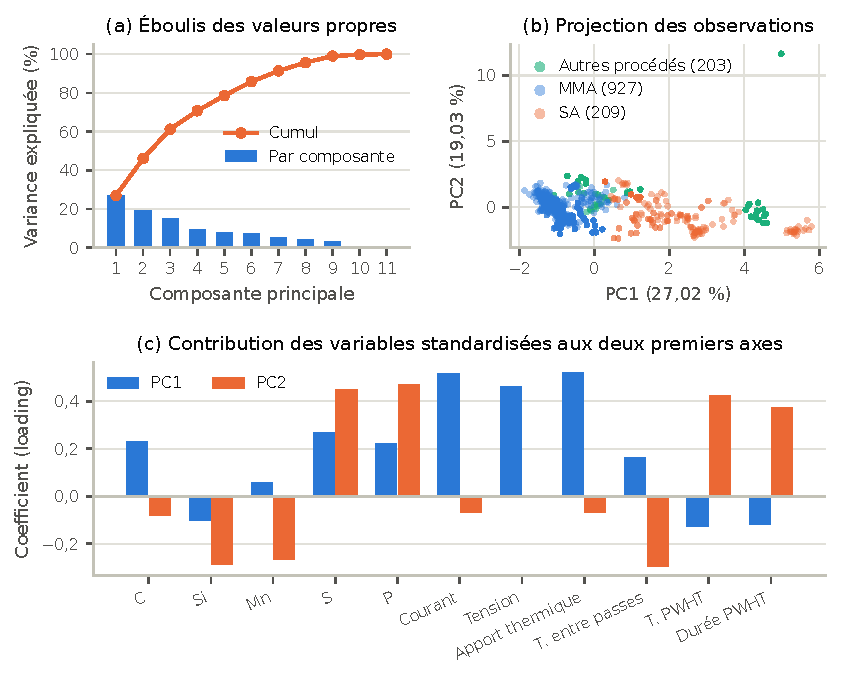
\includegraphics[width=0.86\textwidth]{eda_acp}
\caption{ACP standardisée des onze entrées complètes. (a) Variance expliquée ;
(b) projection sur les deux premiers axes, colorée par procédé ; (c) coefficients
des variables sur les deux premiers axes.}
\label{fig:acp}
\end{figure}

% =====================================================================
\section{Cibles, préparation et protocole}
\label{sec:prep}

\paragraph{Cibles.} YS, UTS et allongement sont les cibles principales (706, 677
et 631 labels dans la cohorte). L'énergie Charpy (861 couples $E(T)$) est
exploratoire : ses protocoles ne sont pas harmonisés entre séries. Aucune cible
n'est imputée.

\paragraph{Préparation.} Le nettoyage est déterministe et traçable : 66\,080
cellules gardent leur valeur brute, leur statut et leur provenance ; \texttt{<L}
est remplacé par $L/2$ et un intervalle par son milieu ; quatre doublons exacts
sont retirés. Les identifiants permettent d'inférer des \textbf{séries
expérimentales}. La cohorte principale retient les lignes qui ont au plus deux
entrées manquantes sur un noyau de 13 variables : \textbf{1\,555 lignes, 44
séries}. Le modèle utilise 16 entrées numériques (C, Si, Mn, S, P, Ni, Cr, Mo,
O, N, courant, tension, apport thermique, température entre passes, température
et durée du PWHT), le procédé et, pour Charpy, la température d'essai.

\paragraph{Prétraitement sans fuite.} Standardisation, encodage one-hot du
procédé et imputation par la médiane sont \textbf{appris dans le seul ensemble
d'entraînement de chaque pli}, au sein d'une pipeline unique. Une première
configuration (13 entrées, imputation itérative) a donné des $R^2$ groupés de
0,02 à 0,19 ; son diagnostic a conduit à ajouter Ni, Cr et Mo (gain de 11 et
9\,MPa de MAE sur YS et UTS) et à passer à la médiane, l'imputation itérative ne
convergeant pas dans 11 contextes.

\paragraph{Validation croisée imbriquée.} Cinq plis externes estiment la
performance ; dans chaque train externe, trois plis internes choisissent la
famille et ses hyperparamètres par MAE~\cite{varma_simon_2006,cawley_talbot_2010}.
Deux scénarios répondent à deux questions :
\begin{itemize}
  \item \textbf{validation aléatoire} (KFold sur les lignes, graine 42) : prédire une soudure d'une série déjà représentée --- 99\,\% des lignes de validation partagent leur série avec le train ;
  \item \textbf{validation groupée} (GroupKFold sur les séries) : prédire une série entièrement nouvelle, le cas d'usage d'une nouvelle étude~\cite{roberts_2017}.
\end{itemize}

\paragraph{Métriques.} Sur $n$ prédictions $\hat{y}_i$ de valeurs $y_i$ de moyenne $\bar{y}$ :
\begin{equation}
  \mathrm{MAE} = \frac{1}{n}\sum_{i=1}^{n}|y_i - \hat{y}_i|, \qquad
  \mathrm{RMSE} = \sqrt{\frac{1}{n}\sum_{i=1}^{n}(y_i - \hat{y}_i)^2}, \qquad
  R^2 = 1 - \frac{\sum_i (y_i - \hat{y}_i)^2}{\sum_i (y_i - \bar{y})^2}.
\end{equation}
La MAE, dans l'unité de la cible et robuste aux valeurs extrêmes, sert à la
sélection ; la RMSE pénalise les grosses erreurs ; le $R^2$, sans unité, compare
les cibles ($R^2 < 0$ : pire que prédire la moyenne). Les scores sont des
moyennes $\pm$ écarts-types sur les cinq plis externes.

% =====================================================================
\section{Méthodes d'apprentissage}
\label{sec:methodes}

\subsection{Méthodes supervisées}

Six familles couvrent des hypothèses différentes sur la relation entre recette
et propriétés (51 configurations réglées par cible et par pli) :
\begin{itemize}
  \item \textbf{médiane de $y$} : référence constante, gain minimal à dépasser ;
  \item \textbf{Ridge}~\cite{hoerl_1970} : régression linéaire pénalisée par $\alpha\lVert\beta\rVert_2^2$, contrôle linéaire ($\alpha$ de 0,01 à 1\,000) ;
  \item \textbf{SVR à noyau RBF}~\cite{smola_2004} : perte $\varepsilon$-insensible et noyau gaussien pour des relations non linéaires lisses ($C$, $\gamma$, $\varepsilon$ réglés ; cible standardisée dans le train) ;
  \item \textbf{forêt aléatoire}~\cite{breiman_2001} : moyenne de 300 arbres sur échantillons bootstrap, qui capte interactions et effets de seuil (taille des feuilles, profondeur, fraction de variables réglées) ;
  \item \textbf{$k$ plus proches voisins}~\cite{cover_1967} : méthode locale ($k \in \{3, 5, 9, 15\}$, distances L1 ou L2), contrôle supervisé de COREG ;
  \item \textbf{XGBoost}~\cite{chen_guestrin_2016} : \emph{boosting} d'arbres, chaque arbre corrigeant les résidus des précédents avec un pas $\eta$ et une pénalité de complexité (profondeur 2 à 6, $\eta \in \{0{,}03; 0{,}1\}$, 150 ou 300 arbres, sans arrêt précoce).
\end{itemize}
Toutes sont implémentées avec scikit-learn~\cite{pedregosa_2011} et XGBoost dans
des notebooks autonomes ; les choix de famille se font uniquement sur la MAE
interne.

\subsection{Méthode semi-supervisée : COREG}

\paragraph{Bibliographie.} Les méthodes semi-supervisées exploitent des entrées
sans label en plus des données étiquetées~\cite{chapelle_2006,vanengelen_2020}.
L'auto-apprentissage (\emph{self-training}) ajoute itérativement les prédictions
les plus sûres d'un modèle comme pseudo-labels~\cite{yarowsky_1995} ; le
co-apprentissage fait échanger ces pseudo-labels entre deux modèles
complémentaires~\cite{blum_mitchell_1998} ; les méthodes de graphe propagent les
labels entre voisins~\cite{zhu_ghahramani_2002}. La plupart ont été conçues pour
la classification, où la confiance d'une prédiction est une probabilité.

\paragraph{Choix et justification.} Nous retenons \textbf{COREG}~\cite{zhou_li_2005},
un co-apprentissage conçu pour la \emph{régression} : deux $k$NN de distances
différentes (L1 et L2) s'échangent des pseudo-labels, et un candidat n'est
accepté que s'il réduit l'erreur locale du modèle sur ses voisins étiquetés. Ce
critère remplace la probabilité, absente en régression. COREG est simple,
inductif (il prédit de nouvelles soudures sans réentraînement) et directement
comparable à son pendant supervisé : la moyenne des deux mêmes $k$NN sans
pseudo-labels isole l'effet des pseudo-labels.

\paragraph{Protocole inductif.} Le pool non étiqueté ne contient que des lignes
de la cohorte sans la cible, prises dans le train du pli (849 à 924 lignes selon
la cible) ; aucune entrée ni aucun label de validation n'est utilisé. COREG est
évalué sur les trois cibles de traction, Charpy n'ayant pas de pool avec
température d'essai connue.

% =====================================================================
\section{Résultats et analyse comparative}
\label{sec:resultats}

\subsection{Procédure supervisée de référence}

Le \cref{tab:synthese} donne le résultat principal : la procédure qui choisit la
famille parmi les six dans la boucle interne.

\begin{table}[!htb]
\centering
\small
\caption{Sélection interne parmi six familles, 16 entrées + procédé, imputation
médiane : moyenne $\pm$ écart-type sur 5 plis externes, et MAE de la référence médiane.}
\label{tab:synthese}
\setlength{\tabcolsep}{3.5pt}
\begin{tabular}{@{}l l rr r r@{}}
\toprule
Cible & Validation & MAE & RMSE & $R^2$ & MAE médiane \\
\midrule
YS (MPa)            & aléatoire & 26,3 $\pm$ 2,7  & 39,1 & 0,82 $\pm$ 0,04 & 70,0 \\
                    & groupée   & 54,4 $\pm$ 9,8  & 70,3 & 0,37 $\pm$ 0,17 & 70,4 \\
UTS (MPa)           & aléatoire & 23,6 $\pm$ 0,8  & 36,5 & 0,83 $\pm$ 0,03 & 68,9 \\
                    & groupée   & 55,7 $\pm$ 12,9 & 70,3 & 0,31 $\pm$ 0,22 & 72,7 \\
Allongement (\%)    & aléatoire & 2,06 $\pm$ 0,22 & 2,89 & 0,65 $\pm$ 0,05 & 4,02 \\
                    & groupée   & 3,28 $\pm$ 0,37 & 4,14 & 0,26 $\pm$ 0,14 & 4,09 \\
Charpy$^*$ (J)      & aléatoire & 14,2 $\pm$ 0,7  & 19,7 & 0,84 $\pm$ 0,03 & 36,8 \\
                    & groupée   & 36,3 $\pm$ 12,8 & 46,4 & 0,06 $\pm$ 0,12 & 36,0 \\
\bottomrule
\end{tabular}
\end{table}

Sur des séries connues, l'erreur typique est de 26\,MPa sur YS et 24\,MPa sur UTS
(4 à 5\,\% de la médiane), soit une MAE réduite de 49 à 66\,\% par rapport à la
référence. Sur des séries nouvelles, l'erreur double et la réduction tombe à
20--23\,\% pour la traction ; pour Charpy, la procédure ne fait pas mieux que la
médiane. \textbf{L'écart entre les deux scénarios est le résultat principal du
projet.}

\subsection{Comparaison des familles}

\begin{figure}[!tb]
\centering
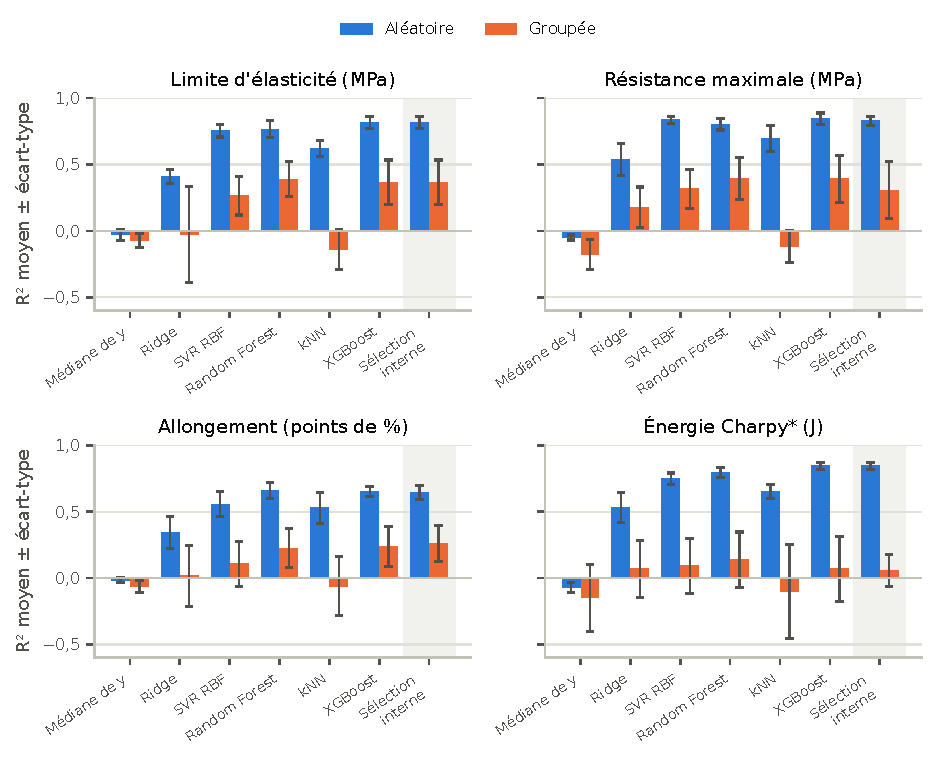
\includegraphics[width=0.72\textwidth]{res_familles_r2}
\caption{$R^2$ moyen ($\pm$ écart-type) de chaque famille réglée en interne et de
la procédure de sélection (fond gris), validations aléatoire (bleu) et groupée (orange).}
\label{fig:familles}
\end{figure}

La \cref{fig:familles} montre que :
\begin{itemize}
  \item \textbf{XGBoost} est la meilleure famille sur des séries connues pour les quatre cibles (MAE de 26,3\,MPa sur YS contre 31,2 pour la forêt) ; la sélection interne le retient dans 17 plis aléatoires sur 20, avec des arbres profonds ;
  \item la \textbf{forêt aléatoire} reste la plus robuste sur des séries nouvelles ($R^2$ de 0,39 sur YS et UTS) ; en groupé, la boucle interne préfère des XGBoost peu profonds (profondeur 2) et choisit même la médiane dans deux plis Charpy ;
  \item \textbf{Ridge} capte peu de signal : la relation n'est pas linéaire ;
  \item le \textbf{$k$NN} est correct en aléatoire mais \emph{négatif} en groupé : une méthode locale réussit quand un voisin de la même série est dans le train, et échoue sinon.
\end{itemize}
L'ajout de XGBoost réduit la MAE de la sélection dans cinq comparaisons sur huit
(YS aléatoire : 31,6 $\rightarrow$ 26,3\,MPa) mais ne change pas la conclusion
groupée. Choisir une famille \emph{après} lecture de ces scores externes serait
une sélection sur la validation : seule la sélection interne est une estimation
honnête.

\subsection{Pourquoi le transfert entre séries échoue}

Une décomposition de l'erreur quadratique de la forêt (premier benchmark groupé)
montre qu'environ \textbf{la moitié de l'erreur} (36 à 56\,\% selon la cible)
vient d'un biais moyen constant sur toute une série : le modèle prédit
correctement les variations à l'intérieur d'une série mais se trompe sur son
niveau. Les prédictions groupées sont \og aplaties \fg{} vers la moyenne. Les
entrées disponibles n'expliquent pas ces décalages, probablement liés à des
éléments non retenus (Nb, V, Ti, B, Cu), à des protocoles d'essai différents ou à
des états métallurgiques non décrits.

\subsection{Apport du semi-supervisé}

\begin{table}[!htb]
\centering
\small
\caption{COREG, son contrôle sans pseudo-labels (deux $k$NN au même $k$) et la
sélection supervisée : MAE moyenne sur 5 plis.}
\label{tab:coreg}
\begin{tabular}{@{}l rrr rrr@{}}
\toprule
 & \multicolumn{3}{c}{Validation aléatoire} & \multicolumn{3}{c}{Validation groupée} \\
\cmidrule(lr){2-4}\cmidrule(lr){5-7}
Cible & COREG & Contrôle & Supervisé & COREG & Contrôle & Supervisé \\
\midrule
YS (MPa)         & 37,9 & 38,2 & \textbf{26,3} & 71,1 & 70,8 & \textbf{54,4} \\
UTS (MPa)        & 33,0 & 33,3 & \textbf{23,6} & 63,1 & 62,1 & \textbf{55,7} \\
Allongement (\%) & 2,40 & 2,39 & \textbf{2,06} & 3,90 & 3,88 & \textbf{3,28} \\
\bottomrule
\end{tabular}
\end{table}

COREG gagne au mieux 0,3\,MPa sur son contrôle en aléatoire, gain non
significatif (intervalles bootstrap par séries couvrant zéro), et perd en groupé
(\cref{tab:coreg}). Il reste 7 à 17\,MPa derrière la sélection supervisée. Trois
raisons sont cohérentes avec ces mesures : les $k$NN de base sont faibles hors
série et COREG ne fait que propager leurs estimations ; le pool provient des
mêmes séries que les labels et apporte peu d'information nouvelle ; enfin tous
les labels disponibles sont déjà utilisés, alors que le semi-supervisé est surtout
utile quand ils sont rares.

% =====================================================================
\section{Des prédictions à une décision : seuils normatifs}
\label{sec:seuils}

Pour juger la qualité d'une soudure, il faut décider si ses propriétés sont
suffisantes. Nos données décrivant surtout du métal fondu, les références
directes sont les normes de classification des consommables, qui imposent
\emph{simultanément} des minimums de traction et de résilience :
ISO 2560-A~\cite{iso_2560,twi_consumables}, ISO 18275-A au-delà de
500\,MPa~\cite{iso_18275}, AWS A5.1 (E7018 : 400\,MPa, 490\,MPa, 22\,\%, 27\,J à
$-29$\,°C)~\cite{aws_a51} et, en offshore, les règles DNV~\cite{dnv_os_c401}.
Ces exigences s'accompagnent de compromis : l'allongement exigé baisse quand la
classe de résistance monte (corrélation YS--allongement de $-0{,}73$ dans nos
données), et un métal fondu plus résistant est plus difficile à rendre
tenace~\cite{keehan_2001,mehmanparast_2018}.

\paragraph{Profil et règle.} Nous retenons la classe \textbf{ISO 2560-A
E~42~2}, au centre de nos données : YS $\geq$ 420\,MPa, UTS $\geq$ 500\,MPa,
allongement $\geq$ 20\,\% et énergie Charpy moyenne $\geq$ 47\,J à $-20$\,°C
(critères critiques), UTS $\leq$ 640\,MPa (informatif). Pour tenir compte de
l'erreur du modèle, nous appliquons la \emph{bande de garde} du
JCGM~106~\cite{jcgm_106} : pour un seuil bas $L$, une prédiction $\hat{y}$ est
conforme (C) si $\hat{y} - 2u \geq L$, non conforme (NC) si $\hat{y} + 2u < L$,
indéterminée (I) sinon, où $u$ est la RMSE hors pli. Avec $w = 2u$, le risque
d'accepter une soudure non conforme est au plus de 2,3\,\% pour une erreur
normale. Une soudure est \textbf{VALIDÉE} si tous ses critères sont C, \textbf{NON
VALIDÉE} si un critère critique est NC, \textbf{PARTIELLE} sinon (essai
nécessaire). Les mesures de la base sont jugées avec $w = 0$ ; chaque soudure
est prédite par un modèle qui ne l'a jamais vue, et l'énergie Charpy à $-20$\,°C.

\begin{figure}[!htb]
\centering
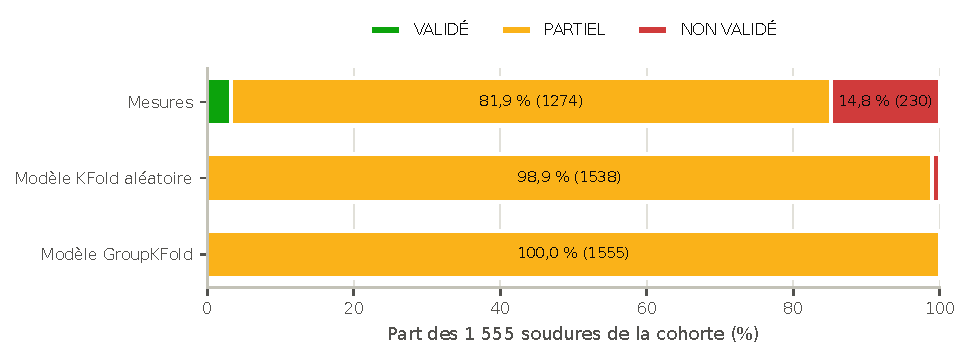
\includegraphics[width=0.95\textwidth]{val_decisions}
\caption{Décisions sur les 1\,555 soudures de la cohorte, profil E~42~2, bande
de garde $2u$ : mesures et prédictions hors pli des deux protocoles.}
\label{fig:validation}
\end{figure}

\paragraph{Résultats.} Les mesures donnent 51 soudures VALIDÉES et 230 NON
VALIDÉES ; les autres sont PARTIELLES, surtout faute de cibles mesurées
ensemble (141 lignes seulement ont les quatre). Le modèle, lui, \textbf{ne valide
aucune soudure} (\cref{fig:validation}) : la plage d'UTS (140\,MPa) est plus
étroite que deux bandes de garde (2 $\times$ 73\,MPa en aléatoire), si bien
qu'aucune prédiction ne peut satisfaire à la fois UTS $\geq$ 500 et UTS $\leq$
640. Ses décisions tranchées sont fiables : par critère, au plus 2,3\,\% de
fausses acceptations dans les deux protocoles, et aucun rejet sur une borne
basse contredit par la mesure. Mais elles sont rares pour une série nouvelle :
le modèle groupé ne tranche que 7 à 27\,\% des critères. En ignorant la borne
haute d'UTS, le modèle aléatoire validerait 125 soudures, dont 2 contredites par
la mesure (1,6\,\%) ; le modèle groupé n'en validerait toujours aucune.

% =====================================================================
\section{Discussion, recommandations et conclusion}
\label{sec:conclusion}

\paragraph{Approche la plus appropriée.} La procédure supervisée --- 16 entrées
et procédé, imputation médiane apprise dans le train, choix de la famille parmi
six par validation interne --- est la plus appropriée ; elle retient surtout
XGBoost. Elle est utile pour \textbf{interpoler dans des séries connues} (erreur
de l'ordre de 25\,MPa sur la résistance), beaucoup moins pour une nouvelle étude
(environ 55\,MPa, $R^2 < 0{,}4$). Les entrées comptent davantage que l'algorithme :
ajouter Ni, Cr et Mo a plus amélioré le transfert que tout changement de famille,
et le semi-supervisé n'apporte pas l'information manquante.

\paragraph{Limites.} La configuration 16/médiane et l'ajout de XGBoost ont été
décidés après les premiers résultats : malgré la validation imbriquée, aucun jeu
indépendant ne confirme la démarche complète. Les séries sont inférées des
identifiants ; Charpy mélange des protocoles ; la règle de validation utilise une
erreur globale par cible plutôt qu'un intervalle propre à chaque soudure, qui
pourrait être obtenu par prédiction conforme~\cite{barber_2021}.

\paragraph{Recommandations pour une bonne qualité de soudure.} Nos modèles
révèlent des associations, pas des causes : nous ne recommandons aucun réglage
\og optimal \fg{} de composition ou de procédé, ce qui demanderait des plans
d'expériences contrôlés. Les données permettent en revanche de recommander :
\begin{enumerate}
  \item de \textbf{mesurer la composition complète}, dont Ni, Cr et Mo, et de documenter le PWHT : ce sont les informations les plus utiles aux modèles de résistance ;
  \item d'\textbf{enregistrer les protocoles d'essai}, en particulier Charpy (courbes $E(T)$ complètes plutôt que températures de transition), et d'identifier séries et publications ;
  \item de \textbf{qualifier chaque soudure par essai} : le modèle sert de filtre avant essai, pas de verdict --- une soudure PARTIELLE vis-à-vis de la classe visée doit être testée ;
  \item de \textbf{valider tout modèle sur de nouvelles séries} et de privilégier la diversité des études plutôt que le nombre de répétitions.
\end{enumerate}

\paragraph{Conclusion.} Prédire les propriétés d'une soudure proche d'une série
connue est réaliste ($R^2$ de 0,65 à 0,85) ; prédire une nouvelle étude reste
difficile ($R^2$ de 0,06 à 0,37), principalement à cause de décalages de niveau
entre séries que les entrées n'expliquent pas. COREG n'améliore pas la
référence supervisée. Face à une exigence normative avec une marge de sécurité,
le modèle trie mais ne qualifie pas : les progrès viendront d'abord de données
plus complètes et mieux documentées.

\medskip
\noindent{\small\textbf{Reproductibilité.} Code dans les notebooks 01 à 09 du
dépôt, 47 tests ciblés ; le rapport complet détaille chaque étape, chaque choix
et l'ensemble des résultats.}

% ---------- Bibliographie -------------------------------------------
{\footnotesize
\setlength{\bibsep}{0.1em}
\bibliographystyle{unsrtnat}
\renewcommand{\refname}{Références bibliographiques}
\bibliography{references}
}

\end{document}
